\chapter{Sprint 3 : virements de masse, contrôles métier et circuit de validation}
\label{ch:sprint3}
\startcontents[chapters]
\chapterplan

\section{Introduction}

Les deux premiers sprints ont fourni les comptes, les sociétés, les fiches de paie et la génération d'un fichier conforme. Le troisième sprint assemble ces briques dans un parcours complet, de la sélection des paiements à la décision du Manager. Il ajoute ce qui distingue SEPAPaie d'un simple générateur de fichiers : des contrôles métier explicites, un suivi des anomalies assorti de recommandations et un circuit de validation fondé sur le principe des quatre yeux. Ce sprint, planifié sur quatre semaines (tableau~\ref{tab:sprints}), concerne les récits US12 à US16.

\section{Backlog du sprint}

\begin{table}[H]
\centering
\footnotesize
\renewcommand{\arraystretch}{1.1}
\tablestyle
\begin{tabularx}{\textwidth}{|>{\centering\arraybackslash}p{0.9cm}|>{\raggedright\arraybackslash}p{5.2cm}|Y|}
\hline
\rowcolor{appMarine}\entete{N\textsuperscript{o}} & \entete{Récit utilisateur} & \entete{Principales tâches} \\
\hline
US12 & Contrôler un virement de masse par des règles métier & Parcours de préparation ; règles sur l'IBAN, le BIC, le montant et les doublons ; restitution des erreurs par salarié \\
\hline
US13 & Consulter et traiter les anomalies avec des recommandations & Registre des anomalies ; statuts et commentaire ; catalogue de recommandations \\
\hline
US14 & Soumettre un fichier au Manager & Conditions de soumission ; statut du fichier ; traçabilité \\
\hline
US15 & Valider ou rejeter un fichier soumis, avec un motif & Liste des fichiers à valider ; principe des quatre yeux ; motif obligatoire au rejet \\
\hline
US16 & Consulter l'historique des fichiers & Historique filtrable ; limitation aux sociétés de l'Expert RH ; vue de supervision de l'administrateur \\
\hline
\end{tabularx}
\caption{Backlog du sprint 3}
\label{tab:backlog-s3}
\end{table}

\section{Conception}

\subsection{Diagramme de cas d'utilisation}

La figure~\ref{fig:uc-s3} présente les cas d'utilisation du sprint. L'Expert RH prépare et contrôle le virement, puis soumet le fichier. Le Manager le valide ou le rejette. Les deux profils métier consultent le résultat, l'historique et traitent les anomalies, alors que l'administrateur se limite à une supervision en lecture seule. L'analyse des montants par l'IA \textbf{étend} le contrôle plutôt que de l'inclure : elle enrichit le résultat lorsqu'elle est disponible, mais son absence n'empêche pas le contrôle d'aboutir.

\begin{figure}[H]
\centering
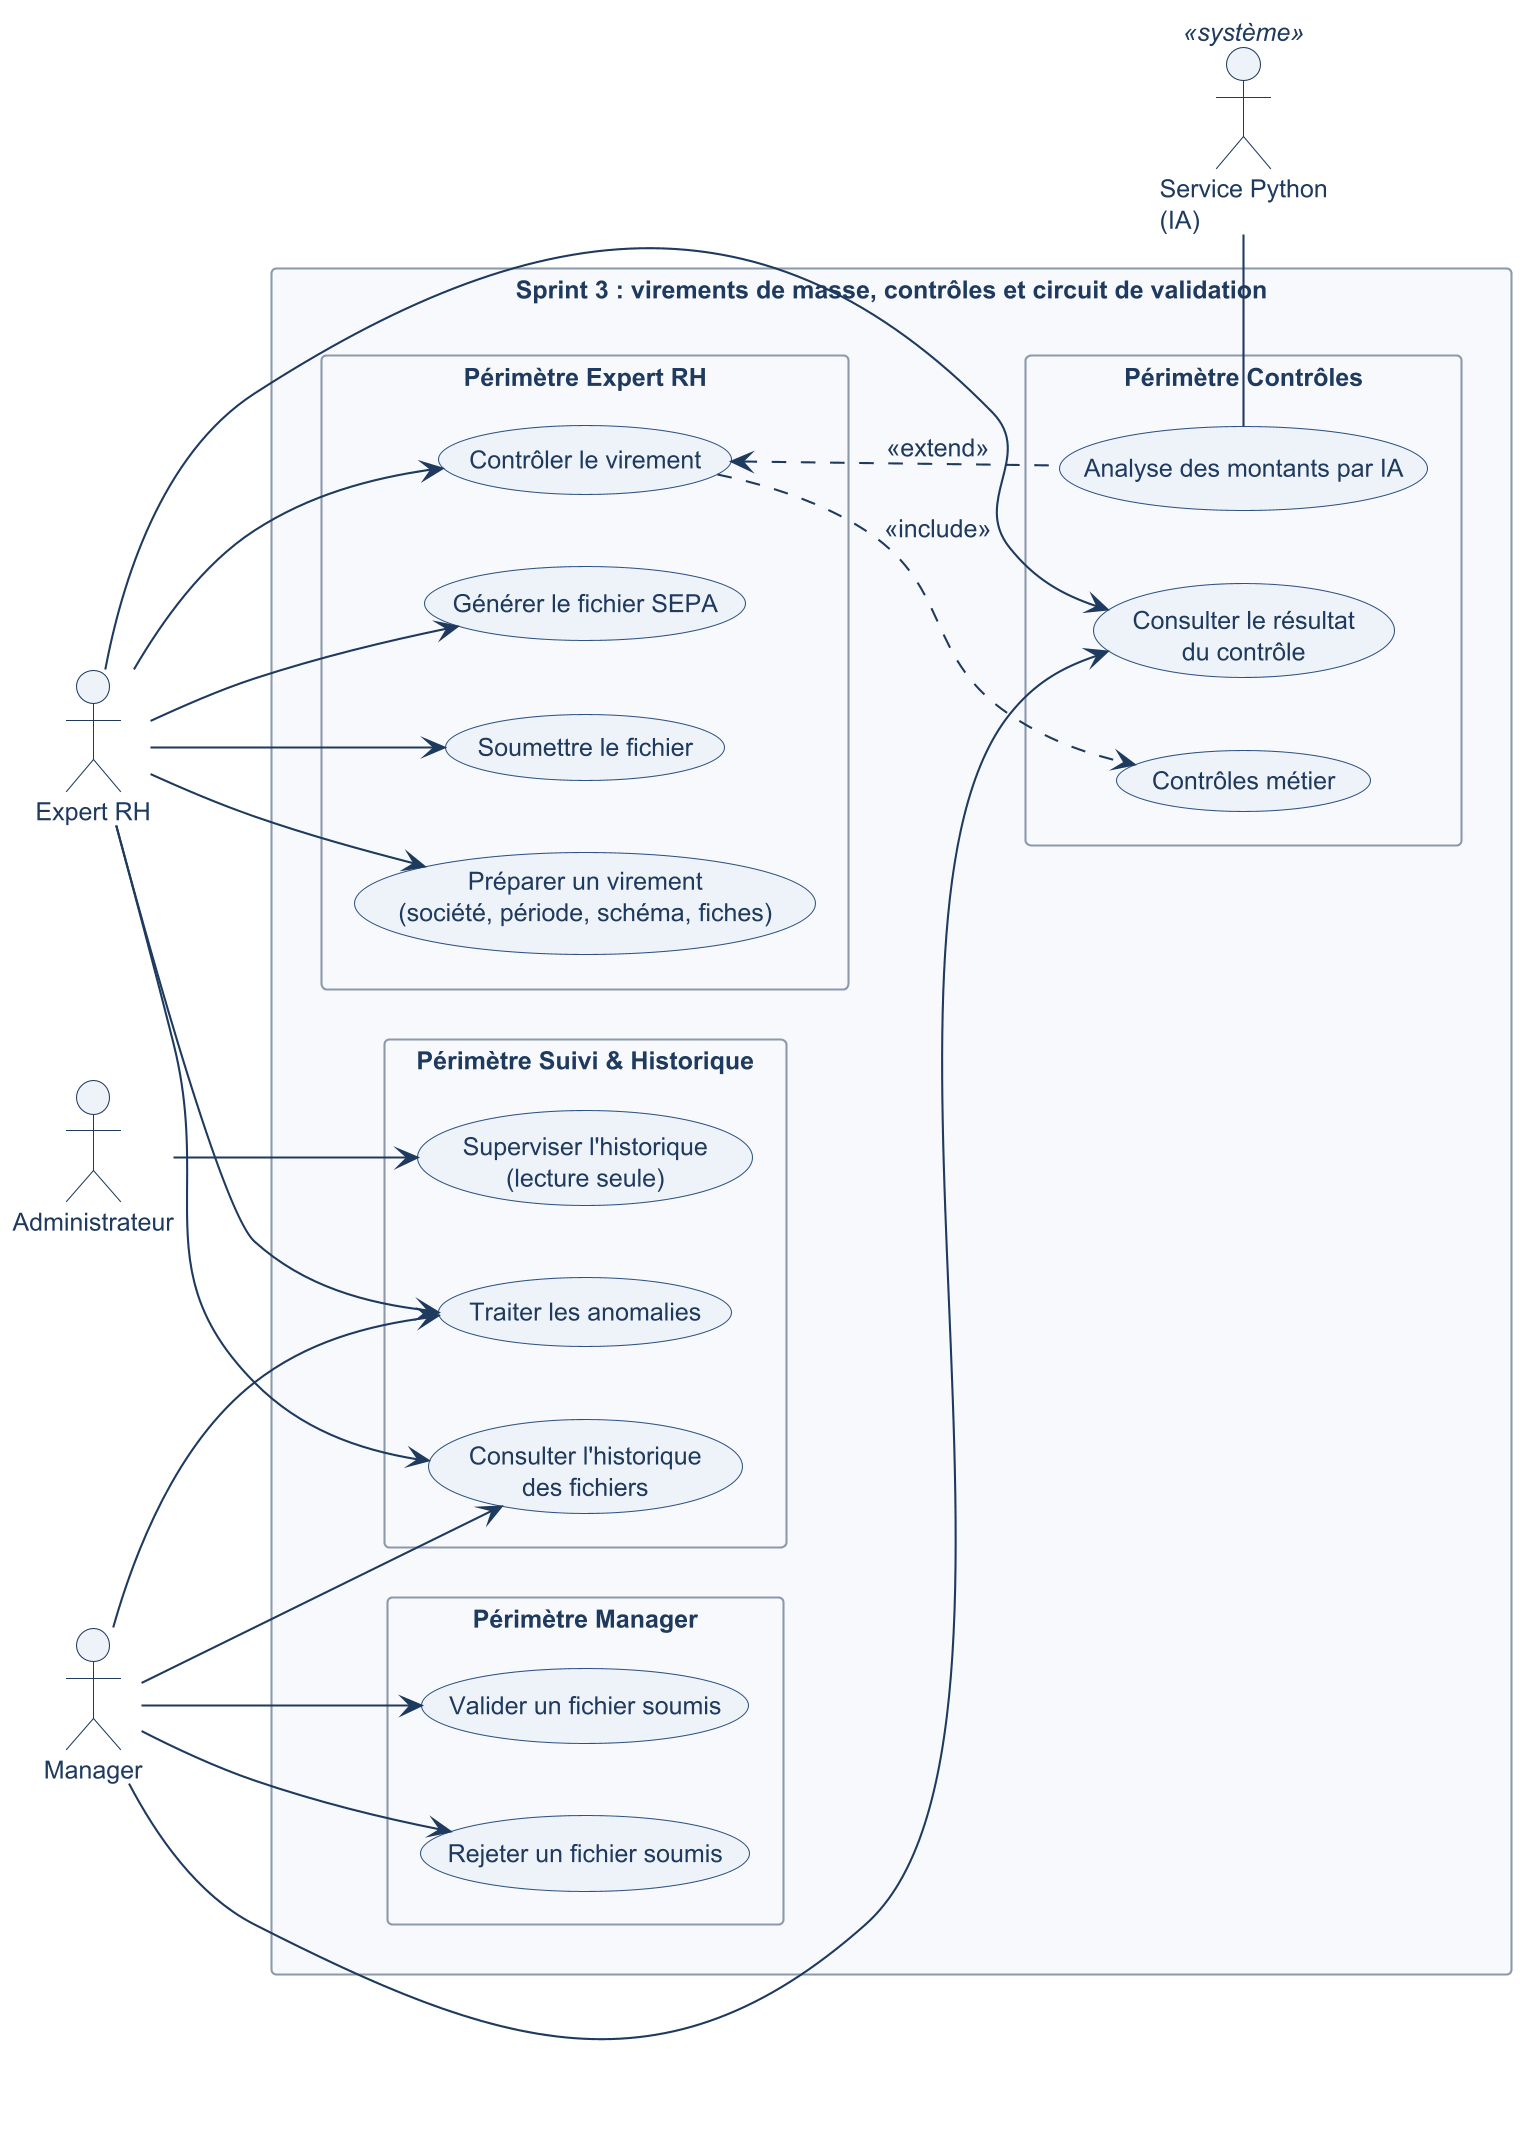
\includegraphics[height=0.4\textheight,width=\textwidth,keepaspectratio]{fig6_1_cas_utilisation_sprint3}
\caption{Cas d'utilisation du sprint 3}
\label{fig:uc-s3}
\end{figure}

\subsection{Parcours en trois étapes}

Le virement de masse est guidé par un parcours en trois étapes affiché en haut de chaque page : la \textbf{préparation}, le \textbf{contrôle} et la \textbf{validation et le téléchargement}. Cette organisation répond à un besoin de lisibilité : l'utilisateur doit savoir à tout moment quelle vérification a été faite et ce qu'il lui reste à traiter. Chaque étape a donc une page dédiée, et le résultat du contrôle est lui-même présenté en cinq onglets : synthèse, XML, validation XSD, contrôle IA et contrôles métier.

\subsection{Cycle de vie d'un fichier}

Un fichier suit un cycle de vie à cinq statuts, illustré par la figure~\ref{fig:etats-fichier}. Le contrôle produit un fichier \og Brouillon\fg{} s'il est conforme au schéma, ou \og Non conforme\fg{} dans le cas contraire. Seul un brouillon peut être soumis. Le Manager décide ensuite : le fichier devient \og Validé par le Manager\fg{} ou \og Rejeté\fg{}. Un fichier rejeté ou non conforme n'est pas corrigé sur place : l'Expert RH relance un nouveau contrôle depuis la préparation, ce qui crée un nouveau fichier et conserve l'ancien dans l'historique.

\begin{figure}[H]
\centering
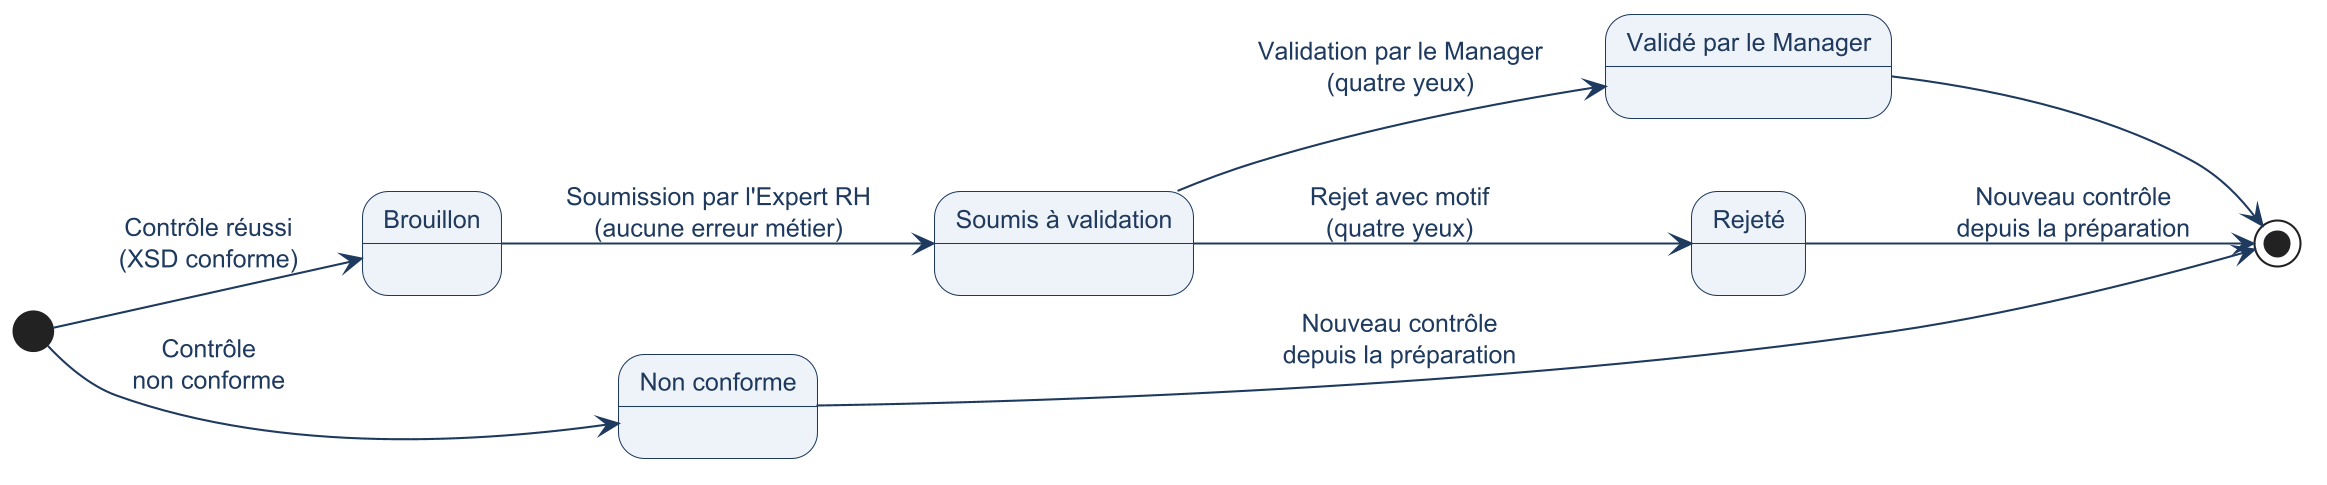
\includegraphics[width=\textwidth]{fig6_2_etats_fichier}
\caption{Cycle de vie d'un fichier SEPA}
\label{fig:etats-fichier}
\end{figure}

Il convient de ne pas confondre ce statut avec celui d'une fiche de paie, décrit au chapitre~\ref{ch:sprint2}. L'approbation concerne un paiement individuel ; la validation concerne le lot soumis. La conformité au schéma XSD, enfin, est une propriété technique du fichier distincte de la décision du Manager.

\subsection{Principe des quatre yeux}

La figure~\ref{fig:seq-validation} décrit la soumission puis la décision. Le principe des quatre yeux s'applique à la décision : la personne qui a généré ou soumis un fichier ne peut ni le valider ni le rejeter. Cette règle est contrôlée par le serveur, et l'interface la reflète en désactivant les boutons et en expliquant pourquoi. Elle s'ajoute à la séparation des rôles : seul un Manager peut décider, et seul un Expert RH peut soumettre.

\begin{figure}[H]
\centering
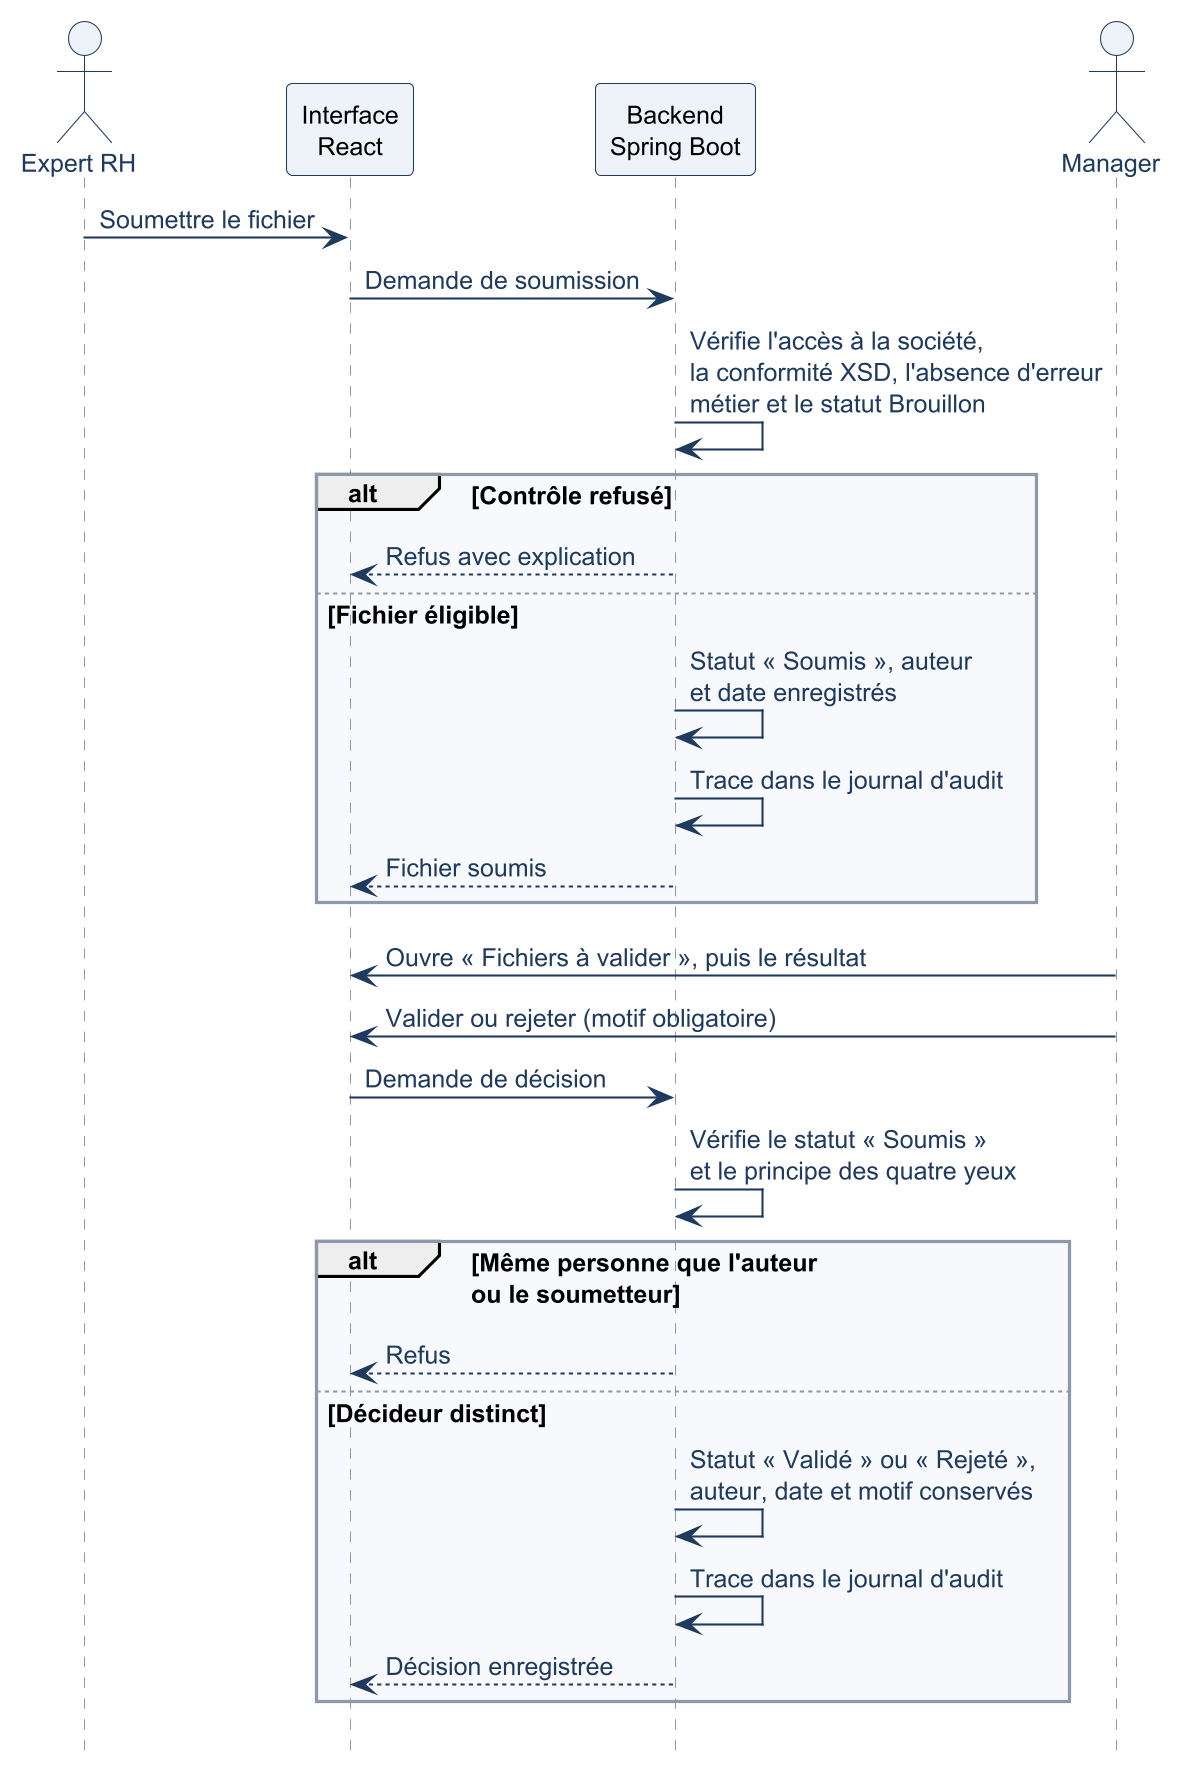
\includegraphics[height=0.5\textheight,width=\textwidth,keepaspectratio]{fig6_3_sequence_validation}
\caption{Séquence de soumission et de décision}
\label{fig:seq-validation}
\end{figure}

\subsection{Préparation d'un virement}

La première page guide l'Expert RH en trois blocs. Il choisit d'abord la \textbf{société débitrice} parmi celles qui lui sont affectées ; l'interface affiche alors sa raison sociale, son BIC et son IBAN masqué, que l'utilisateur peut révéler ponctuellement. Si les coordonnées bancaires de la société sont incomplètes ou si la société est inactive, la génération est bloquée avec un message qui indique ce qu'il faut compléter. Un fichier ne concerne qu'une seule société.

Il renseigne ensuite la période de paie, le schéma XSD et la date d'exécution, proposée par défaut à deux jours ouvrés. Une analyse du schéma choisi peut être consultée. Il examine enfin la liste des paiements approuvés de la société pour la période choisie. Pour chaque paiement, un indicateur affiche le résultat des contrôles de données et, le cas échéant, un signalement de l'IA. Les paiements en erreur sont décochés par défaut, mais restent consultables et peuvent être cochés. L'utilisateur peut filtrer par nom ou matricule et suit en direct le nombre de paiements retenus et leur total (figure~\ref{fig:ecran-preparation}).

Le bouton de lancement reste inactif tant qu'une condition manque, et la page indique laquelle. Une confirmation rappelle le nombre de paiements et le total avant le lancement. Si l'utilisateur quitte la page avec une sélection en cours, l'interface demande confirmation afin d'éviter une perte accidentelle.

\subsection{Lancement du contrôle}

Le lancement déclenche un unique appel au serveur, qui enchaîne dans l'ordre : les contrôles métier, l'analyse par l'IA, la génération du XML puis sa validation contre le schéma. Pendant le traitement, l'interface affiche l'étape en cours. Le résultat est ensuite enregistré dans l'historique, qu'il soit conforme ou non : un fichier non conforme est conservé pour que ses erreurs restent consultables, mais il ne peut être ni téléchargé ni soumis. L'opération est tracée dans le journal d'audit.

Si le service d'IA est désactivé ou indisponible, le traitement se poursuit et le résultat l'indique explicitement (\og Analyse IA indisponible\fg{}). L'absence d'analyse n'est donc jamais confondue avec une absence de risque détecté.

\subsection{Contrôles métier}

Les contrôles métier traduisent des règles explicites sur chaque paiement. Le tableau~\ref{tab:regles-metier} les présente avec leur gravité.

\begin{table}[H]
\centering
\small
\renewcommand{\arraystretch}{1.2}
\tablestyle
\begin{tabularx}{\textwidth}{|>{\raggedright\arraybackslash}p{3.4cm}|Y|>{\centering\arraybackslash}p{2.3cm}|}
\hline
\rowcolor{appMarine}\entete{Contrôle} & \entete{Règle appliquée} & \entete{Gravité} \\
\hline
IBAN & Présence, format général, puis clé de contrôle modulo~97 & Erreur \\
\hline
BIC & Si renseigné : huit ou onze caractères conformes au format attendu & Erreur \\
\hline
Montant & Renseigné et strictement positif & Erreur \\
\hline
Doublon potentiel & Même IBAN et même montant apparaissant plusieurs fois dans la sélection & Avertissement \\
\hline
\end{tabularx}
\caption{Règles de contrôle métier appliquées avant génération}
\label{tab:regles-metier}
\end{table}

Chaque message identifie le paiement par son matricule et indique l'action à mener. Les erreurs sont aussi positionnées sur la ligne du XML correspondante, ce qui permet de passer d'un message à l'élément concerné. Une erreur métier empêche la \textbf{soumission} du fichier, même si le XML est conforme au schéma : la conformité structurelle et l'exactitude des données restent deux vérifications distinctes. L'écran de la figure~\ref{fig:ecran-controles} en donne un exemple.

L'avertissement de doublon ne bloque pas : deux paiements identiques peuvent être légitimes, mais ils méritent une vérification. De même, un montant signalé par l'IA produit un avertissement et non une erreur, comme l'établit le chapitre~\ref{ch:sprint4}.

\subsection{Anomalies et recommandations}

En complément des contrôles lancés sur un fichier, un registre d'anomalies conserve les problèmes détectés sur l'ensemble des fiches de paie. Le tableau~\ref{tab:types-anomalies} en donne les types. Les neuf types déclarés dans l'application ne sont pas tous produits par le registre : les trois derniers sont prévus par le catalogue de recommandations pour d'autres contrôles.

\begin{table}[H]
\centering
\small
\renewcommand{\arraystretch}{1.2}
\tablestyle
\begin{tabularx}{\textwidth}{|>{\raggedright\arraybackslash}p{4.8cm}|Y|}
\hline
\rowcolor{appMarine}\entete{Type d'anomalie} & \entete{Origine et signification} \\
\hline
\texttt{IBAN\_INVALIDE} & Règle métier : IBAN absent, mal formé ou à clé incorrecte \\
\hline
\texttt{BIC\_INVALIDE} & Règle métier : BIC renseigné mais mal formé \\
\hline
\texttt{MONTANT\_INVALIDE} & Règle métier : montant nul ou négatif \\
\hline
\texttt{DOUBLON\_PAIEMENT} & Règle métier : plusieurs fiches avec le même IBAN et le même montant \\
\hline
\texttt{IBAN\_PARTAGE} & Règle métier : un même IBAN utilisé par plusieurs salariés \\
\hline
\texttt{MONTANT\_SUSPECT} & Module d'IA : montant atypique, avec ses raisons \\
\hline
\texttt{NET\_SUPERIEUR\_BRUT},\newline \texttt{ERREUR\_XSD},\newline \texttt{CTRL\_SUM\_INCOHERENT} & Types prévus par le catalogue de recommandations, non alimentés par la détection actuelle \\
\hline
\end{tabularx}
\caption{Types d'anomalies du registre}
\label{tab:types-anomalies}
\end{table}

Une anomalie a un statut de suivi : \textbf{ouverte}, \textbf{corrigée} ou \textbf{ignorée}. Les deux profils métier peuvent la marquer corrigée ou l'ignorer ; l'ignorer exige un commentaire, qui garde la trace du motif. La détection peut être relancée à la demande. Elle réconcilie le registre avec l'état actuel des fiches : une nouvelle anomalie est créée, une anomalie qui n'est plus détectée passe à \og corrigée\fg{}, et une anomalie corrigée à la main qui réapparaît est rouverte. Les anomalies ignorées ne sont pas modifiées. Si l'IA est indisponible lors d'une détection, les anomalies d'origine IA restent ouvertes au lieu d'être classées à tort comme corrigées.

Chaque anomalie reçoit à sa création une \textbf{recommandation} tirée d'un catalogue par type. Le texte s'appuie sur les valeurs réelles : matricule, IBAN masqué, montant et période. Par exemple, pour un IBAN invalide, la recommandation conseille de demander un RIB à jour au salarié, de corriger l'IBAN puis de relancer la génération. En cas d'incident du moteur de recommandation, un message générique est utilisé afin de ne jamais interrompre la détection. La figure~\ref{fig:ecran-anomalies} montre le registre.

Le registre est partagé par les deux profils métier, mais l'Expert RH ne voit que les anomalies des fiches de ses sociétés et ne peut modifier le statut que de celles-ci ; le Manager voit l'ensemble.

\subsection{Soumission et décision}

La \textbf{soumission}, réservée à l'Expert RH, exige quatre conditions : l'accès à la société du fichier, la conformité au schéma, l'absence d'erreur de contrôle métier et le statut \og Brouillon\fg{}. Elle enregistre l'auteur et la date, trace l'événement dans le journal d'audit et fait passer le fichier au statut \og Soumis à validation\fg{}. Lorsque le fichier comporte une erreur métier, le serveur refuse la soumission et l'interface masque le bouton en indiquant la raison (figure~\ref{fig:ecran-synthese}).

Le Manager retrouve les fichiers soumis dans une liste dédiée, triée du plus ancien au plus récent. Il ouvre le résultat complet, puis valide ou rejette (figure~\ref{fig:ecran-decision}). Le rejet exige un motif, qui est conservé et affiché ensuite à l'Expert RH. Dans les deux cas, le statut, l'auteur de la décision et sa date sont enregistrés et le journal d'audit en garde la trace. Seul un fichier soumis peut être validé ou rejeté.

Le statut conditionne aussi le téléchargement. Un fichier validé est téléchargé sous son nom d'origine. Tout autre téléchargement reçoit le préfixe \og NON\_VALIDE\fg{}, afin qu'un fichier de contrôle ne soit pas confondu avec un fichier destiné à la banque. SEPAPaie ne transmet pas le fichier à la banque : cette étape reste hors du périmètre.

\subsection{Historique et supervision}

L'historique recense les fichiers avec leur date, leur société, leur période, le nombre de salariés, le total, la conformité XSD, le résultat de l'IA, le statut et l'auteur. Il se filtre par statut et par recherche libre. Un Expert RH n'y voit que les fichiers de ses sociétés ; le Manager les voit tous. L'administrateur dispose d'une \textbf{vue de supervision} en lecture seule : il suit l'activité, mais ne voit ni les matricules, ni les motifs de rejet, ni les acteurs du circuit, et ne dispose d'aucune action (figure~\ref{fig:ecran-supervision}).

\subsection{Interfaces réalisées}

La figure~\ref{fig:ecran-preparation} présente la préparation d'un virement par un Expert RH. La liste affiche les contrôles de chaque paiement : la fiche EMP002 du jeu de démonstration porte un IBAN dont la clé est incohérente, ce qui est signalé en rouge.

\begin{figure}[H]
\centering
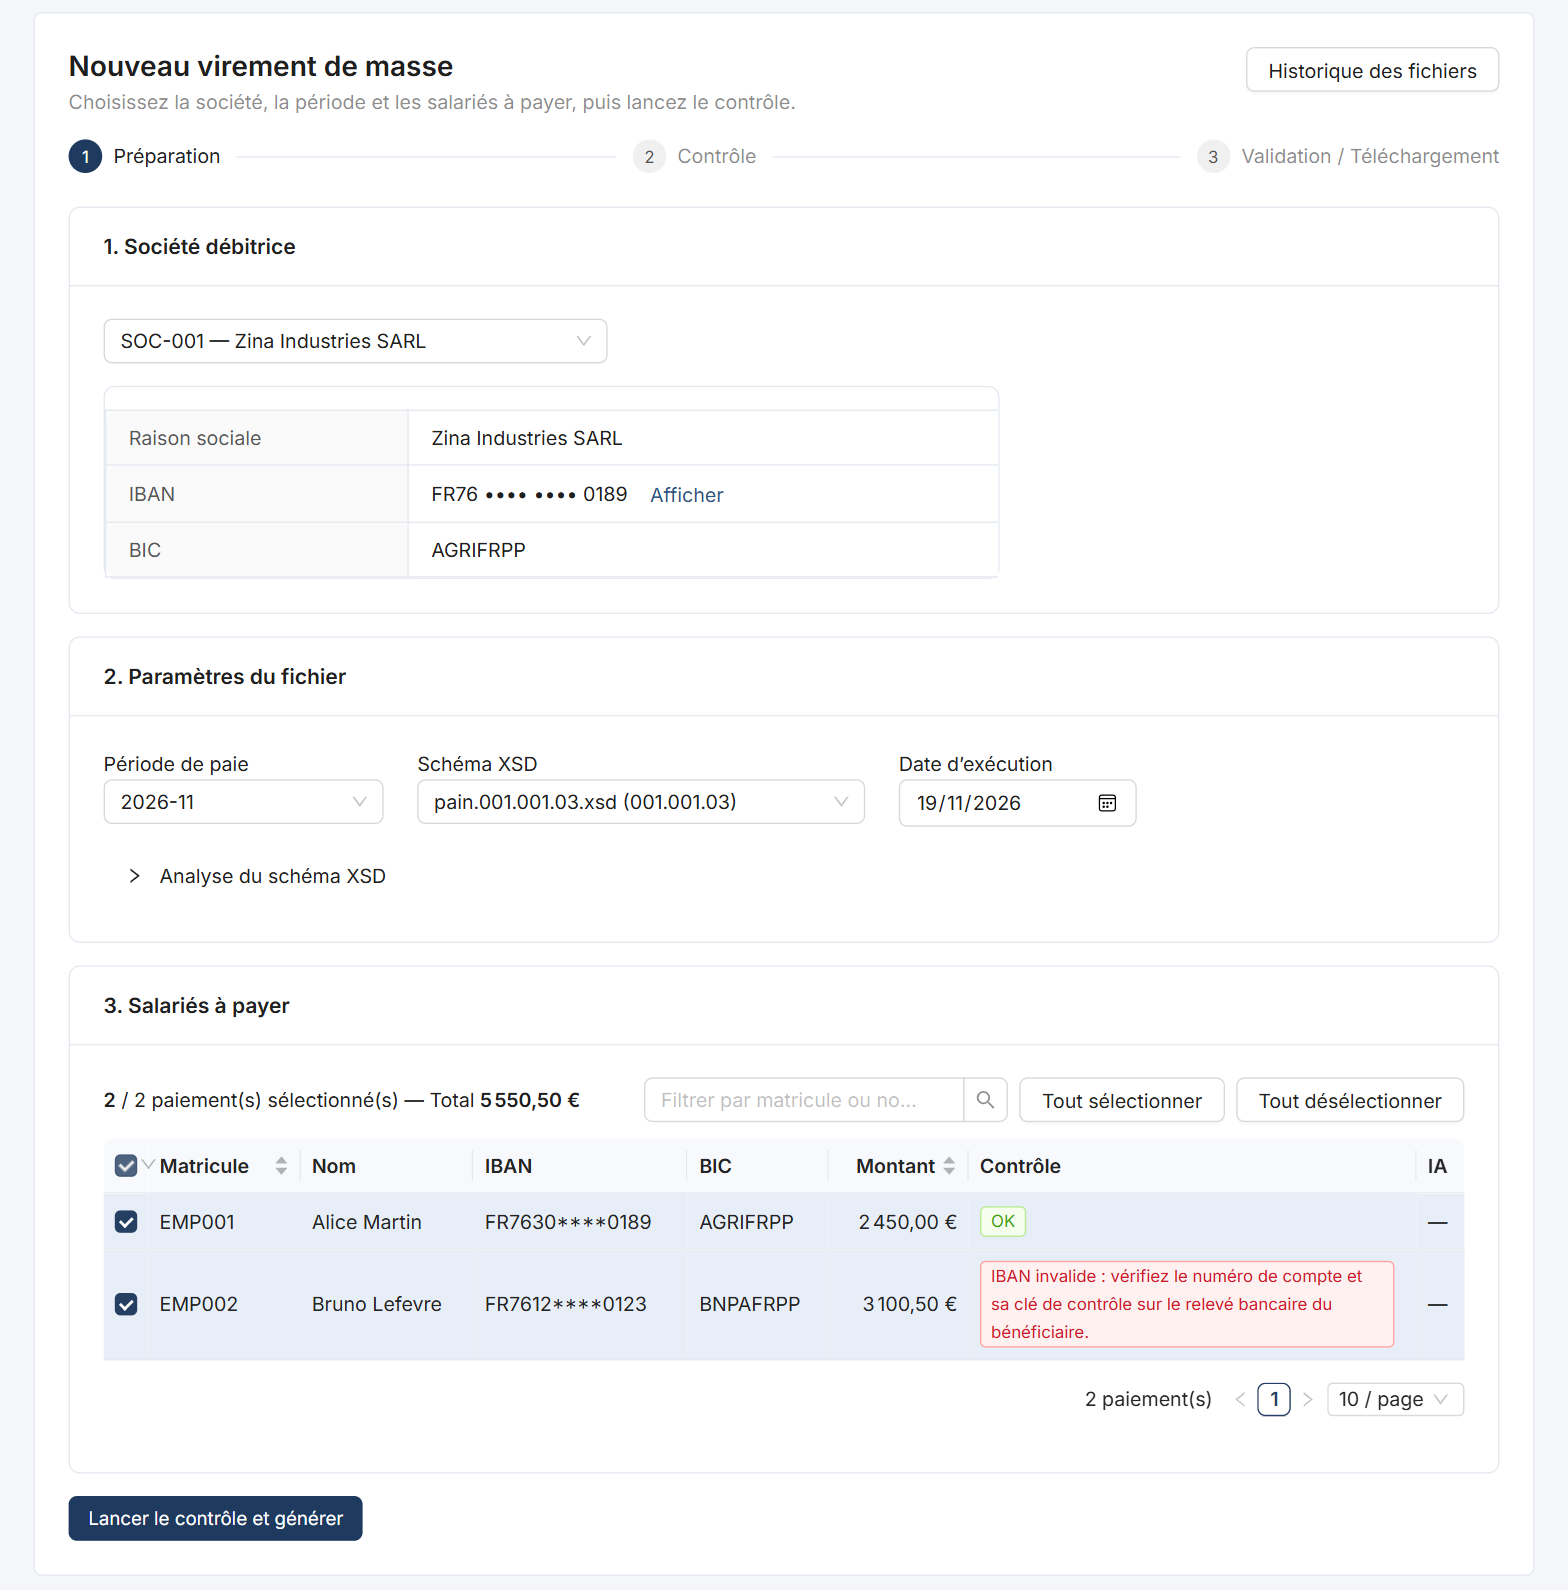
\includegraphics[width=0.95\textwidth]{fig6_preparation}
\caption{Préparation d'un virement de masse (profil Expert RH)}
\label{fig:ecran-preparation}
\end{figure}

La figure~\ref{fig:ecran-synthese} montre la synthèse du résultat. Les cartes résument les quatre dimensions du contrôle : validation XSD, contrôles métier, contrôle IA et statut du fichier. Ici, l'erreur métier bloque la soumission, et le message l'explique. La figure~\ref{fig:ecran-controles} détaille cette erreur dans l'onglet dédié.

\begin{figure}[H]
\centering
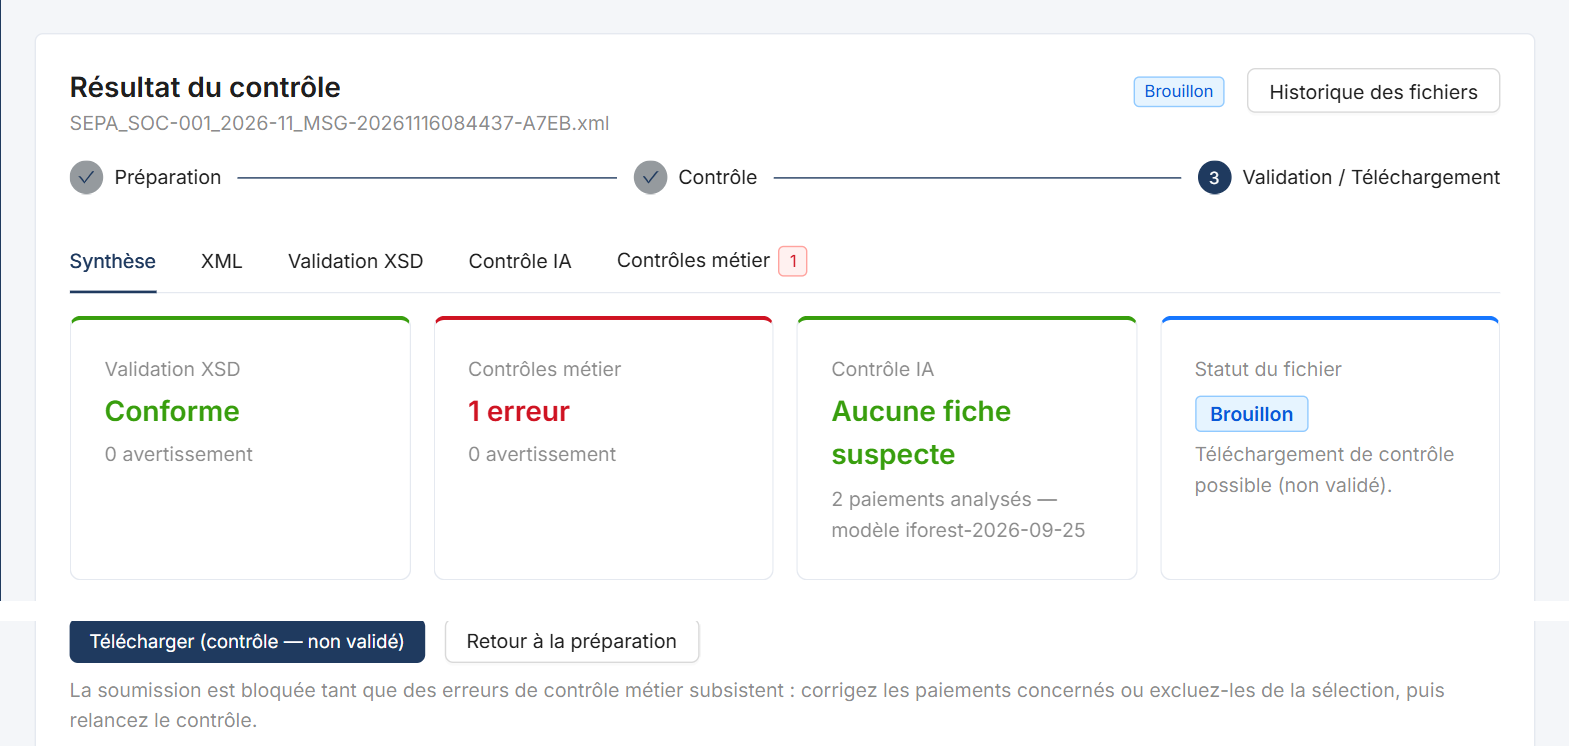
\includegraphics[width=0.95\textwidth]{fig6_synthese}
\caption{Synthèse du résultat : soumission bloquée par une erreur métier}
\label{fig:ecran-synthese}
\end{figure}

\begin{figure}[H]
\centering
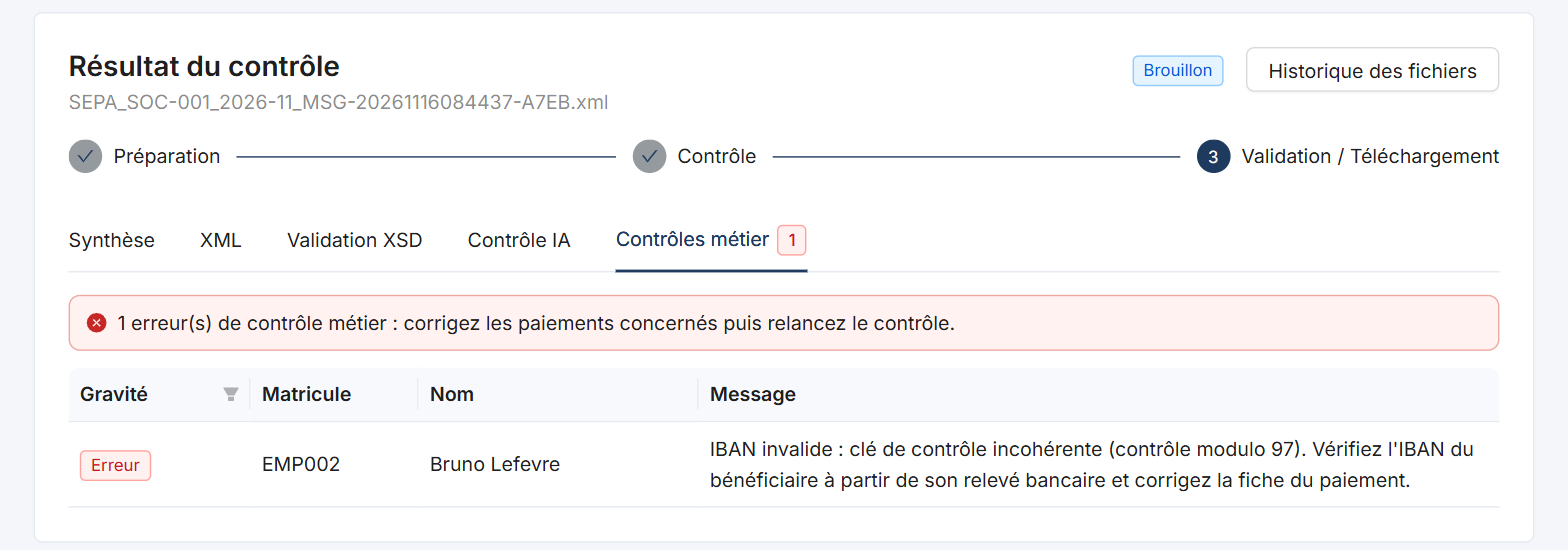
\includegraphics[width=0.95\textwidth]{fig6_controles_metier}
\caption{Onglet des contrôles métier}
\label{fig:ecran-controles}
\end{figure}

Après la soumission, le Manager ouvre le résultat du fichier : les boutons de validation et de rejet apparaissent sous le résultat (figure~\ref{fig:ecran-decision}). La figure~\ref{fig:ecran-supervision} montre la vue de supervision de l'administrateur, sans actions ni détail par salarié.

\begin{figure}[H]
\centering
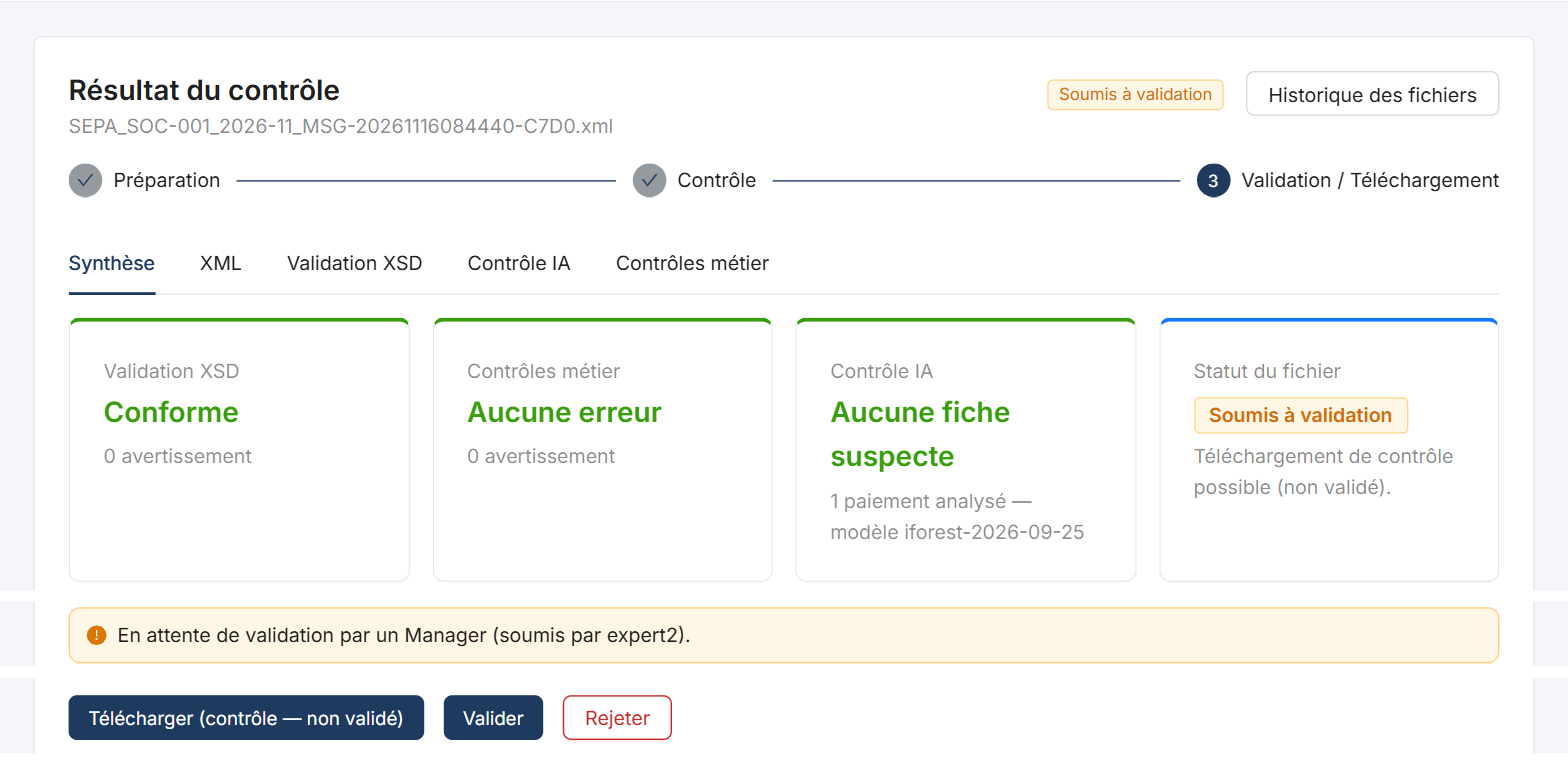
\includegraphics[width=0.95\textwidth]{fig6_decision}
\caption{Fichier soumis : décision du Manager}
\label{fig:ecran-decision}
\end{figure}

\begin{figure}[H]
\centering
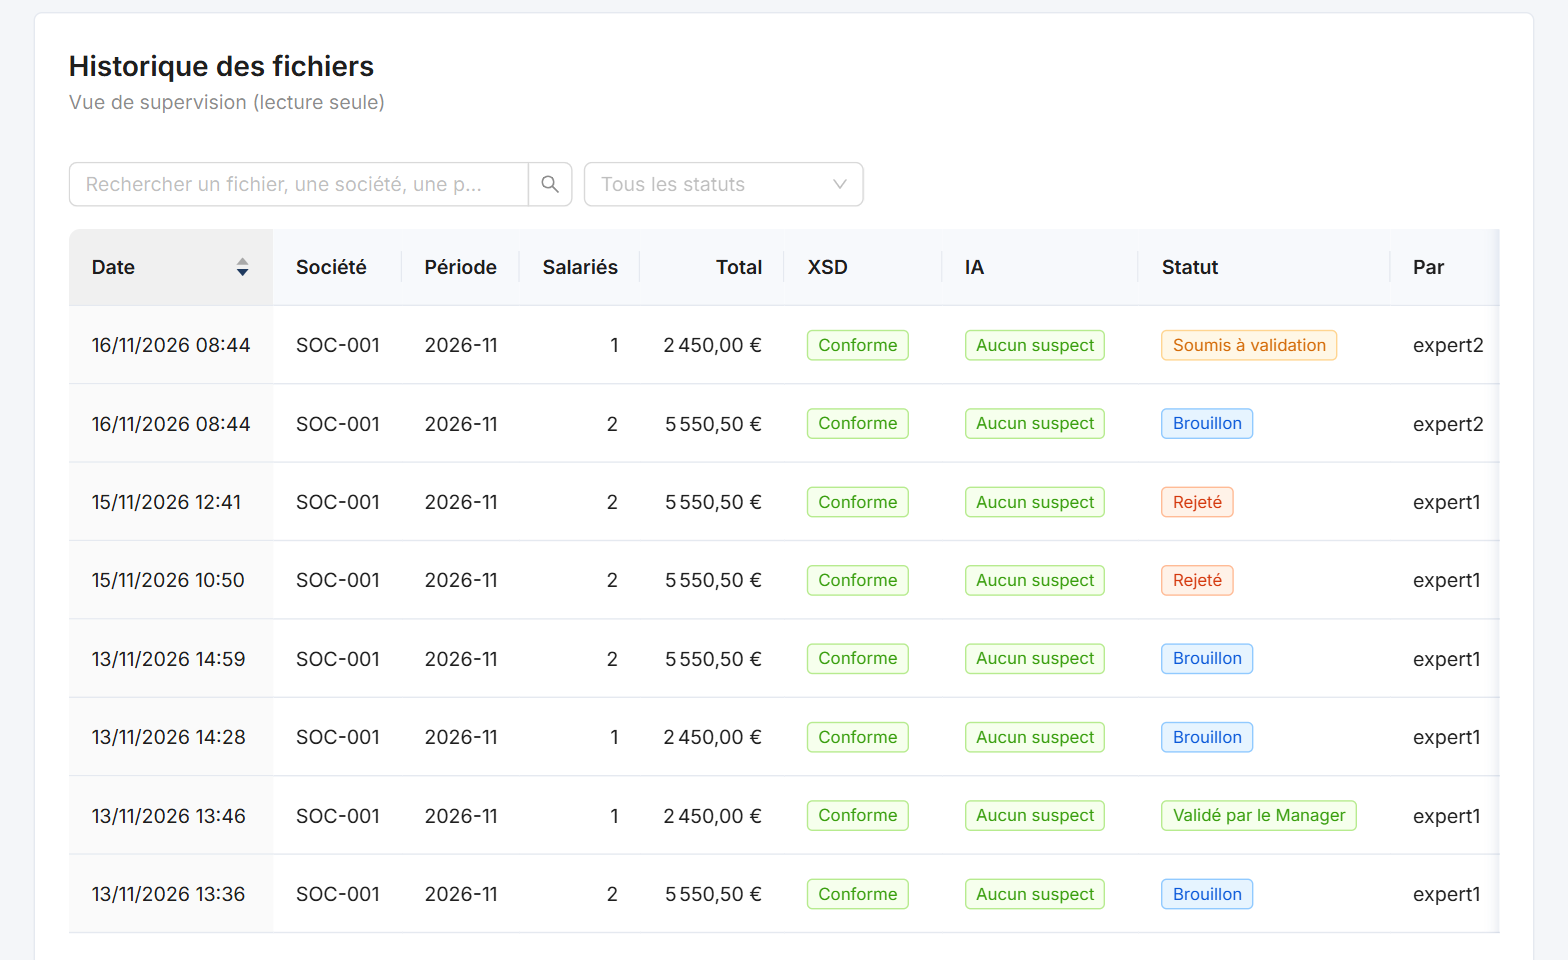
\includegraphics[width=0.95\textwidth]{fig6_supervision}
\caption{Vue de supervision de l'historique (profil administrateur)}
\label{fig:ecran-supervision}
\end{figure}

Enfin, la figure~\ref{fig:ecran-anomalies} présente le registre des anomalies avec leurs recommandations et leurs actions de suivi.

\begin{figure}[H]
\centering
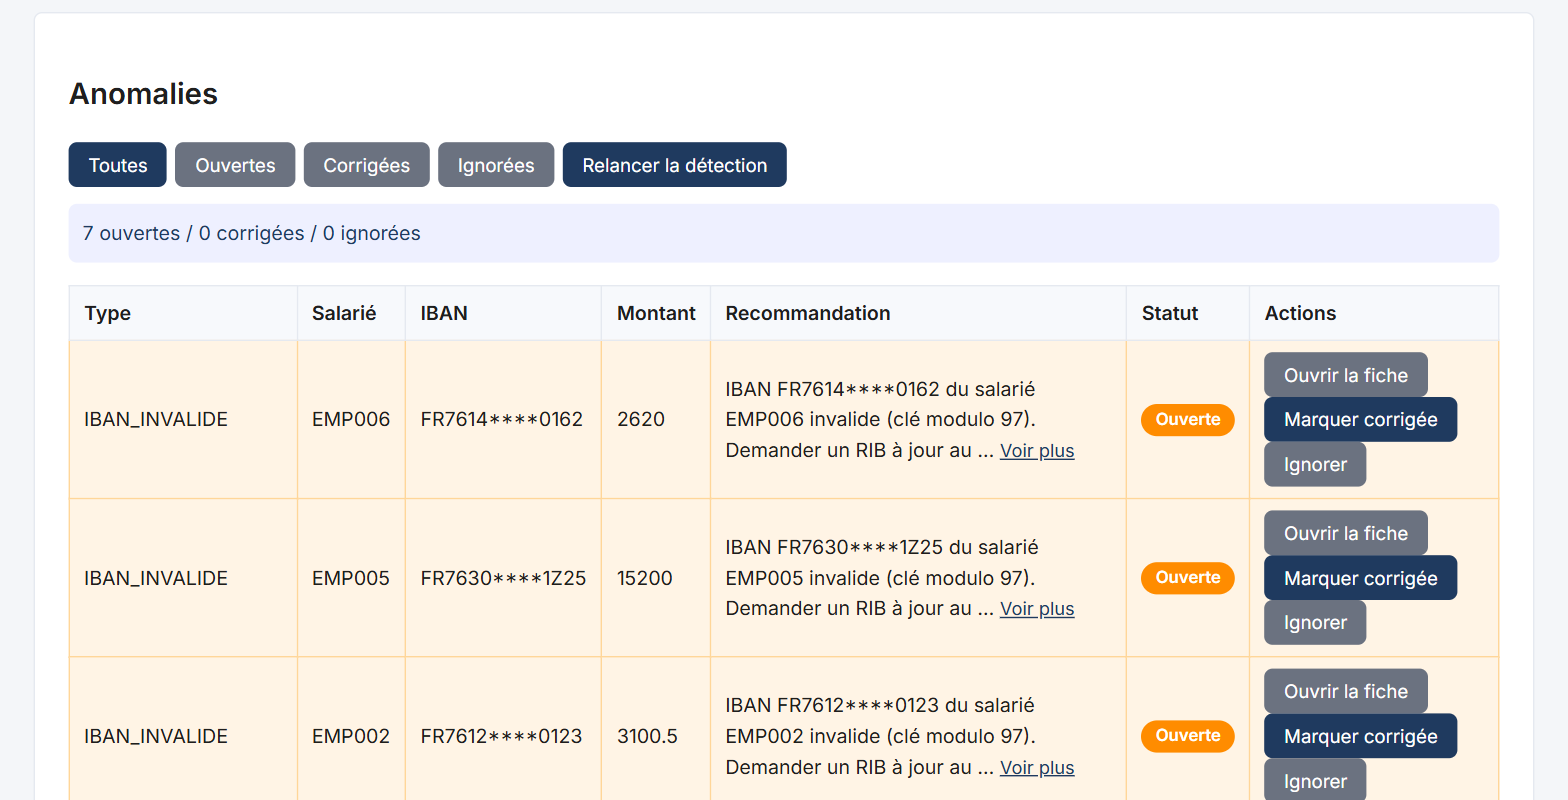
\includegraphics[width=0.95\textwidth]{fig6_anomalies}
\caption{Registre des anomalies (profil Manager)}
\label{fig:ecran-anomalies}
\end{figure}

\section{Conclusion}

Le sprint 3 a assemblé les briques précédentes en un parcours de virement de masse complet : préparation guidée, contrôles métier, génération et validation, suivi des anomalies avec recommandations, puis circuit de décision fondé sur les quatre yeux. Les fichiers non conformes ou comportant des erreurs de données ne peuvent pas être soumis, et chaque étape est tracée. Le chapitre suivant présente le sprint 4, consacré à la détection d'anomalies par intelligence artificielle, à son intégration et à son évaluation.

